\documentclass[]{article}
\usepackage{lmodern}
\usepackage{amssymb,amsmath}
\usepackage{ifxetex,ifluatex}
\usepackage{fixltx2e} % provides \textsubscript
\ifnum 0\ifxetex 1\fi\ifluatex 1\fi=0 % if pdftex
  \usepackage[T1]{fontenc}
  \usepackage[utf8]{inputenc}
\else % if luatex or xelatex
  \ifxetex
    \usepackage{mathspec}
  \else
    \usepackage{fontspec}
  \fi
  \defaultfontfeatures{Ligatures=TeX,Scale=MatchLowercase}
\fi
% use upquote if available, for straight quotes in verbatim environments
\IfFileExists{upquote.sty}{\usepackage{upquote}}{}
% use microtype if available
\IfFileExists{microtype.sty}{%
\usepackage{microtype}
\UseMicrotypeSet[protrusion]{basicmath} % disable protrusion for tt fonts
}{}
\usepackage[margin=1in]{geometry}
\usepackage{hyperref}
\hypersetup{unicode=true,
            pdftitle={MXB262 Practical 1: Introduction to R, ggplot2, and Rmarkdown},
            pdfauthor={MXB262 QUT},
            pdfborder={0 0 0},
            breaklinks=true}
\urlstyle{same}  % don't use monospace font for urls
\usepackage{color}
\usepackage{fancyvrb}
\newcommand{\VerbBar}{|}
\newcommand{\VERB}{\Verb[commandchars=\\\{\}]}
\DefineVerbatimEnvironment{Highlighting}{Verbatim}{commandchars=\\\{\}}
% Add ',fontsize=\small' for more characters per line
\usepackage{framed}
\definecolor{shadecolor}{RGB}{248,248,248}
\newenvironment{Shaded}{\begin{snugshade}}{\end{snugshade}}
\newcommand{\AlertTok}[1]{\textcolor[rgb]{0.94,0.16,0.16}{#1}}
\newcommand{\AnnotationTok}[1]{\textcolor[rgb]{0.56,0.35,0.01}{\textbf{\textit{#1}}}}
\newcommand{\AttributeTok}[1]{\textcolor[rgb]{0.77,0.63,0.00}{#1}}
\newcommand{\BaseNTok}[1]{\textcolor[rgb]{0.00,0.00,0.81}{#1}}
\newcommand{\BuiltInTok}[1]{#1}
\newcommand{\CharTok}[1]{\textcolor[rgb]{0.31,0.60,0.02}{#1}}
\newcommand{\CommentTok}[1]{\textcolor[rgb]{0.56,0.35,0.01}{\textit{#1}}}
\newcommand{\CommentVarTok}[1]{\textcolor[rgb]{0.56,0.35,0.01}{\textbf{\textit{#1}}}}
\newcommand{\ConstantTok}[1]{\textcolor[rgb]{0.00,0.00,0.00}{#1}}
\newcommand{\ControlFlowTok}[1]{\textcolor[rgb]{0.13,0.29,0.53}{\textbf{#1}}}
\newcommand{\DataTypeTok}[1]{\textcolor[rgb]{0.13,0.29,0.53}{#1}}
\newcommand{\DecValTok}[1]{\textcolor[rgb]{0.00,0.00,0.81}{#1}}
\newcommand{\DocumentationTok}[1]{\textcolor[rgb]{0.56,0.35,0.01}{\textbf{\textit{#1}}}}
\newcommand{\ErrorTok}[1]{\textcolor[rgb]{0.64,0.00,0.00}{\textbf{#1}}}
\newcommand{\ExtensionTok}[1]{#1}
\newcommand{\FloatTok}[1]{\textcolor[rgb]{0.00,0.00,0.81}{#1}}
\newcommand{\FunctionTok}[1]{\textcolor[rgb]{0.00,0.00,0.00}{#1}}
\newcommand{\ImportTok}[1]{#1}
\newcommand{\InformationTok}[1]{\textcolor[rgb]{0.56,0.35,0.01}{\textbf{\textit{#1}}}}
\newcommand{\KeywordTok}[1]{\textcolor[rgb]{0.13,0.29,0.53}{\textbf{#1}}}
\newcommand{\NormalTok}[1]{#1}
\newcommand{\OperatorTok}[1]{\textcolor[rgb]{0.81,0.36,0.00}{\textbf{#1}}}
\newcommand{\OtherTok}[1]{\textcolor[rgb]{0.56,0.35,0.01}{#1}}
\newcommand{\PreprocessorTok}[1]{\textcolor[rgb]{0.56,0.35,0.01}{\textit{#1}}}
\newcommand{\RegionMarkerTok}[1]{#1}
\newcommand{\SpecialCharTok}[1]{\textcolor[rgb]{0.00,0.00,0.00}{#1}}
\newcommand{\SpecialStringTok}[1]{\textcolor[rgb]{0.31,0.60,0.02}{#1}}
\newcommand{\StringTok}[1]{\textcolor[rgb]{0.31,0.60,0.02}{#1}}
\newcommand{\VariableTok}[1]{\textcolor[rgb]{0.00,0.00,0.00}{#1}}
\newcommand{\VerbatimStringTok}[1]{\textcolor[rgb]{0.31,0.60,0.02}{#1}}
\newcommand{\WarningTok}[1]{\textcolor[rgb]{0.56,0.35,0.01}{\textbf{\textit{#1}}}}
\usepackage{longtable,booktabs}
\usepackage{graphicx,grffile}
\makeatletter
\def\maxwidth{\ifdim\Gin@nat@width>\linewidth\linewidth\else\Gin@nat@width\fi}
\def\maxheight{\ifdim\Gin@nat@height>\textheight\textheight\else\Gin@nat@height\fi}
\makeatother
% Scale images if necessary, so that they will not overflow the page
% margins by default, and it is still possible to overwrite the defaults
% using explicit options in \includegraphics[width, height, ...]{}
\setkeys{Gin}{width=\maxwidth,height=\maxheight,keepaspectratio}
\IfFileExists{parskip.sty}{%
\usepackage{parskip}
}{% else
\setlength{\parindent}{0pt}
\setlength{\parskip}{6pt plus 2pt minus 1pt}
}
\setlength{\emergencystretch}{3em}  % prevent overfull lines
\providecommand{\tightlist}{%
  \setlength{\itemsep}{0pt}\setlength{\parskip}{0pt}}
\setcounter{secnumdepth}{0}
% Redefines (sub)paragraphs to behave more like sections
\ifx\paragraph\undefined\else
\let\oldparagraph\paragraph
\renewcommand{\paragraph}[1]{\oldparagraph{#1}\mbox{}}
\fi
\ifx\subparagraph\undefined\else
\let\oldsubparagraph\subparagraph
\renewcommand{\subparagraph}[1]{\oldsubparagraph{#1}\mbox{}}
\fi

%%% Use protect on footnotes to avoid problems with footnotes in titles
\let\rmarkdownfootnote\footnote%
\def\footnote{\protect\rmarkdownfootnote}

%%% Change title format to be more compact
\usepackage{titling}

% Create subtitle command for use in maketitle
\providecommand{\subtitle}[1]{
  \posttitle{
    \begin{center}\large#1\end{center}
    }
}

\setlength{\droptitle}{-2em}

  \title{MXB262 Practical 1: Introduction to R, ggplot2, and Rmarkdown}
    \pretitle{\vspace{\droptitle}\centering\huge}
  \posttitle{\par}
    \author{MXB262 QUT}
    \preauthor{\centering\large\emph}
  \postauthor{\par}
      \predate{\centering\large\emph}
  \postdate{\par}
    \date{2020}


\begin{document}
\maketitle

\hypertarget{this-week}{%
\subsection{This Week}\label{this-week}}

This week you will learn how to:

\begin{enumerate}
\def\labelenumi{\arabic{enumi}.}
\setcounter{enumi}{-1}
\tightlist
\item
  download R, RStudio, and start writing some code
\item
  use Rmarkdown to make nice and accessible documents with text, code
  chunks, and figures\\
\item
  set the working directory\\
\item
  create a simple plot using \texttt{plot()}
\item
  load R packages
\item
  use \texttt{ggplot()} to visualise data
\end{enumerate}

\hypertarget{obtaining-r}{%
\subsection{0. Obtaining R}\label{obtaining-r}}

R can be downloaded from \url{http://cran.r‐project.org/} Using a script
editor, such as ``RStudio,'' can also be helpful. RStudio can be
downloaded from \url{http://www.rstudio.com/}

\hypertarget{starting-rstudio}{%
\subsection{Starting RStudio}\label{starting-rstudio}}

Click the RStudio icon to open RStudio. The interface is divided into
several panels (clockwise From top left):

\begin{enumerate}
\def\labelenumi{\arabic{enumi}.}
\tightlist
\item
  The source code (supporting tabs)
\item
  The currently active objects/history
\item
  A File browser/plot window/package install window/R help window
  (tabbed)
\item
  The R console The source code editor (top left) is where you type,
  edit and save your R code.
\end{enumerate}

The source code editor (top left) is where you type, edit and save your
R code. The editor supports text highlighting, autocompletes common
functions and parentheses, and allows the user to select R code and run
it in the R console (bottom right) with a keyboard shortcut (Ctrl R on
windows, command-enter on macs). Code will appear in this font:

\begin{verbatim}
plot(x,y)
\end{verbatim}

\hypertarget{starting-a-new-script}{%
\subsection{Starting a new script}\label{starting-a-new-script}}

Let's open a new script and save it to your harddrive. In matlab, this
is the equivalent to an `m file'. Instead of typing every command into
the console, making a script lets you record and save everything that
you do. So next week if you're wondering how you made that line plot, or
did that calculation, or ran that multi-line simulation, you can just
pull up the R script and run it exactly the same. Remember that
\#dataviz is about reproducibility -- using scripts in R is one step
toward that goal.

When writing R scripts, use lots of \# comments throughout your R
scripts to record what you were thinking or what the code does. Any line
or text that starts with \# won't run, it's just there to communicate
with whoever reads your code later. Usually that is you, but sometimes
it will be your tutors or your collaborators. If you liberally use
comments you will thank yourself when you go back to the analysis later!

Similarly at the start of your script, put some meta-information about
the whole script, such as: \# who wrote the code? \# what does the code
do? \# when did you write the code? etc.

The more projects you work on and analyses you do, the more important it
is to have this meta- information at the beginning of your code. Every
academic and data scientist wishes they were just a little bit better at
doing this, so start now.

\begin{center}\rule{0.5\linewidth}{\linethickness}\end{center}

\hypertarget{r-markdown}{%
\subsection{1. R Markdown}\label{r-markdown}}

This is an R Markdown document. In MXB262 all assignments and worksheets
will be completed in this format. Markdown is a simple formatting syntax
for authoring HTML, PDF, and MS Word documents. For more details on
using R Markdown see \url{http://rmarkdown.rstudio.com}.

When you click the \textbf{Knit} button (at the top of the Editor window
in RStudio -- it helpfully has a little ball of wool and knitting
needles next to it), a document will be generated that includes the
content, figures, and the output of any embedded R code chunks within
the document. This is useful because then everything is in one place --
you only need to make one document with your text, code, and figures,
not create a Word doc and continually copy updated code, results, and
figures into it.

The real magic of an R Markdown script is that you can embed an R code
chunk like this:

\begin{Shaded}
\begin{Highlighting}[]
\KeywordTok{plot}\NormalTok{(cars)}
\end{Highlighting}
\end{Shaded}

\includegraphics{W2_introtoR_worksheet_files/figure-latex/cars-1.pdf}

In the knitted pdf, you'll see the code (```\{`plot(cars)'\}), plus the
output from the code (the figure). In the source code (i.e.~the script),
you'll just see the code, but when you press the green `play' button
next to it the figure will show up.

Creating headers, tables, lists and indentations is easy, you can find a
cheat sheet here
\url{https://www.rstudio.com/wp-content/uploads/2015/02/rmarkdown-cheatsheet.pdf}.
Save the cheat sheet to your desktop or print it out so you have it on
hand for the workshops (or do what I do, and google it every single
time).

You're going to be using R Markdown for all worksheets, Problem Solving
tasks 1-6, and the summaries of your projects. If you are having
troubles with R Markdown at any point, please ask your tutor in
practicals or via email, or you won't be able to submit your assessment.

\hypertarget{task}{%
\paragraph{TASK}\label{task}}

\begin{quote}
\begin{enumerate}
\def\labelenumi{\arabic{enumi}.}
\tightlist
\item
  Update the author (your name) and date fields at the top of this file.
\end{enumerate}
\end{quote}

\begin{quote}
\begin{enumerate}
\def\labelenumi{\arabic{enumi}.}
\setcounter{enumi}{1}
\tightlist
\item
  Use the knit button to render the file to pdf.\\
\item
  Run the code in only the individual chunk above, instead of the full
  document, by clicking the \emph{Run} button inside the chunk (the
  green arrow to the right of the `````\{r cars\}'' line). Or, run each
  line of code one by one in the console by placing your cursor inside
  the chunk and pressing \emph{Cmd+Shift+Enter}.
\end{enumerate}
\end{quote}

\begin{center}\rule{0.5\linewidth}{\linethickness}\end{center}

\hypertarget{adding-code-chunks}{%
\subsection{2. Adding code chunks}\label{adding-code-chunks}}

\hypertarget{task-1}{%
\paragraph{TASK}\label{task-1}}

\begin{quote}
\begin{enumerate}
\def\labelenumi{\arabic{enumi}.}
\setcounter{enumi}{3}
\tightlist
\item
  Add a new code chunk by clicking the \emph{Insert R} button on the
  toolbar or by pressing \emph{Cmd+Option+I} for mac or
  \emph{ctrl+alt+I} for pc.
\item
  Within that code chunk add a new plot using the \texttt{plot()}
  function, and the dataset \texttt{discoveries}
\end{enumerate}
\end{quote}

Note: the \texttt{echo\ =\ FALSE} parameter can be added to the code
chunk to prevent the R code that generated the plot from being printed.
Like this:

\includegraphics{W2_introtoR_worksheet_files/figure-latex/pressure-1.pdf}

When you pressed knit, you only saw the figure -- not the code that
generated it (look back up in the html file to the cars plot -- you can
see the code was printed for that one).

\begin{center}\rule{0.5\linewidth}{\linethickness}\end{center}

\hypertarget{setting-the-working-directory}{%
\subsection{3. Setting the working
directory}\label{setting-the-working-directory}}

To use R you will to access data, save files, and sometimes access
images. The folder that stores all documents for a project is called the
\texttt{working\ directory}. R needs to know where to look for data
files and/or where to save generated files, that is, where the
\texttt{working\ directory} for this project is. Follow the following
steps to set-up the working directory for MXB262.

\begin{enumerate}
\def\labelenumi{\arabic{enumi}.}
\tightlist
\item
  In the console use the \texttt{setwd("add\ file\ path\ here")}
  function to set the working directory to a file of your choice. You
  must keep the " " marks inside the brackets.
\item
  Type the \texttt{getwd()} function in the console to check that
  returned file path is correct.
\end{enumerate}

\textbf{NOTE: Please do not submit any code that contains the
\texttt{setwd()} function. Please either just set it on your computer
each time you open R Studio, or comment the line of code out by placing
a \# in front of the code. If you include it, when the tutor is trying
to mark your code it will try to reorganise the files on the tutor's
computer. This can make marking very difficult!}

\begin{center}\rule{0.5\linewidth}{\linethickness}\end{center}

\hypertarget{data}{%
\subsection{4. Data}\label{data}}

This unit is all about data visualisation, which means we need data. To
make this easy to start with, we will be using data that is already
clean, ready to use and available within R. See
\href{https://stat.ethz.ch/R-manual/R-devel/library/datasets/html/00Index.html}{package}
for a list of all datasets already loaded into R.

\hypertarget{task-2}{%
\paragraph{TASK}\label{task-2}}

\begin{quote}
\begin{enumerate}
\def\labelenumi{\arabic{enumi}.}
\setcounter{enumi}{4}
\tightlist
\item
  Create a new chunk and add a plot of one of the datasets listed on the
  (\href{https://stat.ethz.ch/R-manual/R-devel/library/datasets/html/00Index.html}{R
  data packages} webpage. Use the \texttt{plot()} function that we
  already used in the code chunk above.
\end{enumerate}
\end{quote}

\begin{center}\rule{0.5\linewidth}{\linethickness}\end{center}

\hypertarget{loading-packages}{%
\subsection{5. Loading packages}\label{loading-packages}}

Packages in R can contain functions as well as data. R comes with some
base packages when you first install it, but if you wish to use
additional packages you need to \emph{install} and then \emph{load}
them.

To install a package use the \texttt{install.package("package\_name")}
function (do this on every new computer), and to load the package use
\texttt{library(package\_name)} (do this every time you re-open R).

Use the code chunk below to install and load the \emph{ggplot2} library.
Note that the first line is commented out using \texttt{\#} to stop the
\texttt{install.packages()} function being run everytime the document is
rendered. You will need to delete the \texttt{\#} and run both lines. I
suggest you add the \texttt{\#} back in once you have successfully
installed ggplot2.

\begin{Shaded}
\begin{Highlighting}[]
\CommentTok{#install.packages("ggplot2")}
\KeywordTok{library}\NormalTok{(ggplot2)}
\end{Highlighting}
\end{Shaded}

\begin{center}\rule{0.5\linewidth}{\linethickness}\end{center}

\hypertarget{visualisation-in-r---ggplot}{%
\subsection{6. Visualisation in R -
ggplot()}\label{visualisation-in-r---ggplot}}

Throughout these practicals we'll be using Hadley Wickham's
\texttt{Grammar\ of\ Graphics} package (more commonly called
\texttt{ggplot2}). You have installed this in the code chunk above.
ggplot2 has a specific format for creating plots, graphs and other
visualisations. Once you understand the format, making and customising
graphics is intuitive.

You can think of building a plot like building a house, the essential
ingredients are: the building materials (your data) and a floor plan
(called the geom in ggplot). After the house is built you can add
fittings and fixtures like taps, door handles, and the house number
(title, labels, change the colours).

\begin{longtable}[]{@{}lll@{}}
\toprule
\begin{minipage}[b]{0.30\columnwidth}\raggedright
house\strut
\end{minipage} & \begin{minipage}[b]{0.31\columnwidth}\raggedright
plot\strut
\end{minipage} & \begin{minipage}[b]{0.30\columnwidth}\raggedright
ggplot function\strut
\end{minipage}\tabularnewline
\midrule
\endhead
\begin{minipage}[t]{0.30\columnwidth}\raggedright
Building Materials\strut
\end{minipage} & \begin{minipage}[t]{0.31\columnwidth}\raggedright
Your data set and which variables in the dataset to use\strut
\end{minipage} & \begin{minipage}[t]{0.30\columnwidth}\raggedright
\texttt{ggplot(dataset,\ aes(x\ =\ variable,\ y\ =\ variable)}\strut
\end{minipage}\tabularnewline
\begin{minipage}[t]{0.30\columnwidth}\raggedright
Floor plan\strut
\end{minipage} & \begin{minipage}[t]{0.31\columnwidth}\raggedright
what type of \texttt{geom} (graph or plot)\strut
\end{minipage} & \begin{minipage}[t]{0.30\columnwidth}\raggedright
\texttt{+\ geom\_point()}\strut
\end{minipage}\tabularnewline
\begin{minipage}[t]{0.30\columnwidth}\raggedright
Fittings and fixtures\strut
\end{minipage} & \begin{minipage}[t]{0.31\columnwidth}\raggedright
add a title, change axis labels, add colours etc\strut
\end{minipage} & \begin{minipage}[t]{0.30\columnwidth}\raggedright
\texttt{+\ ggtitle()} \texttt{+\ ylab()}, \texttt{+\ xlab()} etc\strut
\end{minipage}\tabularnewline
\begin{minipage}[t]{0.30\columnwidth}\raggedright
Add it all together\strut
\end{minipage} & \begin{minipage}[t]{0.31\columnwidth}\raggedright
\strut
\end{minipage} & \begin{minipage}[t]{0.30\columnwidth}\raggedright
\texttt{ggplot(dataset,\ aes(x\ =\ variable,\ y\ =\ variable)\ +\ geom\_bar()\ +\ ggtitle()}\strut
\end{minipage}\tabularnewline
\bottomrule
\end{longtable}

The following code chunk re-creates the pressure plot above but using
ggplot.

\begin{Shaded}
\begin{Highlighting}[]
\CommentTok{# 1. Load ggplot2 library/package}
\KeywordTok{library}\NormalTok{(ggplot2)}

\CommentTok{# 2. The building materials are: ggplot(pressure, aes(x= temperature, y = pressure)) }
\CommentTok{# 3. Define the floor/graph plan (tell ggplot which type of graph to make) : + geom_point()}
\CommentTok{# 4. Add titles and axis labels: ggtitle("Go forth and create awesome data visualisations") + ylab("Take the pressure down") + xlab("It's getting hot in here")}
\CommentTok{# 5. Assign the plot to an object called 'scatterplot_house'}

\NormalTok{scatterplot_house <-}\StringTok{ }\KeywordTok{ggplot}\NormalTok{(pressure, }\KeywordTok{aes}\NormalTok{(}\DataTypeTok{x=}\NormalTok{ temperature, }\DataTypeTok{y =}\NormalTok{ pressure)) }\OperatorTok{+}\StringTok{ }\KeywordTok{geom_point}\NormalTok{() }\OperatorTok{+}\StringTok{ }\KeywordTok{ggtitle}\NormalTok{(}\StringTok{"Go forth and create awesome data visualisations"}\NormalTok{) }\OperatorTok{+}\StringTok{ }\KeywordTok{ylab}\NormalTok{(}\StringTok{"Take the pressure down"}\NormalTok{) }\OperatorTok{+}\StringTok{ }\KeywordTok{xlab}\NormalTok{(}\StringTok{"It's getting hot in here"}\NormalTok{)}

\CommentTok{#print the plot}
\NormalTok{scatterplot_house}
\end{Highlighting}
\end{Shaded}

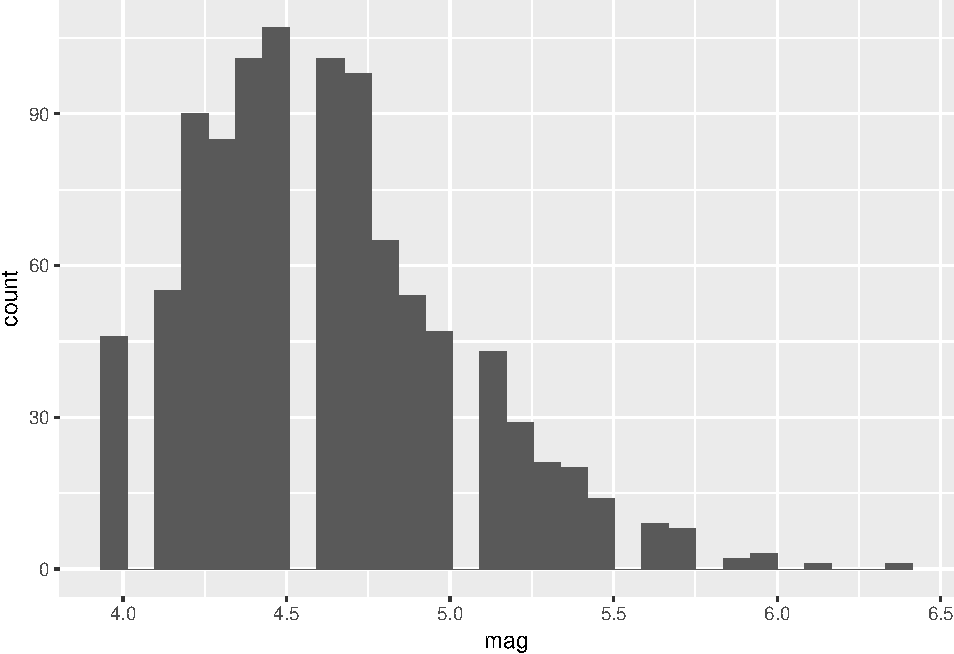
\includegraphics{W2_introtoR_worksheet_files/figure-latex/unnamed-chunk-2-1.pdf}

A cheat sheet for ggplot can be found
\url{https://www.rstudio.com/wp-content/uploads/2015/03/ggplot2-cheatsheet.pdf}.

We will be using Hadley Wickham's free online book
\href{https://r4ds.had.co.nz/.html}{R for Data Science} to learn more
about ggplot. You can start at Chapter 3 Data Visualisation, however the
introductory chapters may also be useful if you are interested in
starting there outside of class time.

\hypertarget{tasks}{%
\paragraph{TASKS}\label{tasks}}

\begin{quote}
\begin{enumerate}
\def\labelenumi{\arabic{enumi}.}
\setcounter{enumi}{5}
\tightlist
\item
  Work through
  \href{https://r4ds.had.co.nz/data-visualisation.html}{Chapter 3 of R
  for Data Science}. Read and follow all the examples along in your own
  R console for sections:
\end{enumerate}
\end{quote}

\begin{itemize}
\tightlist
\item
  3.1
\item
  3.2 (including all exercises)
\item
  3.3 (and exercises 1-3)
\item
  3.4
\item
  3.5 (skip these exercises in class)
\item
  3.6 (skip these exercises).
\end{itemize}

You can go back to the exercises you skipped outside of class time,
although they aren't critical at this stage of the unit.

\begin{quote}
\begin{enumerate}
\def\labelenumi{\arabic{enumi}.}
\setcounter{enumi}{6}
\tightlist
\item
  Work through (i.e.~use the code to generate for yourself) the first 3
  plots in \href{http://varianceexplained.org/r/trump-tweets/}{Donald
  Trump's twitter example} that we talked about in the lecture. Although
  all of the code here is useful, pay particular attention to the ggplot
  commands being used here. These are all simple, but well-chosen and
  effective plots. NOTE: you will need to install the twitteR package
  first. You won't be able to set up the Twitter authentication, so
  ignore the second code chunks on the website -- start by downloading
  the dataset by running the third code chunk. Once they start getting
  into the word analysis, they stop walking us through the
  visualisations. Code for those figures follows here, so keep following
  and running all of the analysis and data-wrangling on the blog but
  jump back to grab this code when you reach each of these questions and
  figures:
\end{enumerate}
\end{quote}

What were the most common words in Trump's tweets overall?

\begin{Shaded}
\begin{Highlighting}[]
\NormalTok{tweet_words }\OperatorTok
\KeywordTok{count}\NormalTok{(word, }\DataTypeTok{sort =} \OtherTok{TRUE}\NormalTok{) }\OperatorTok
\KeywordTok{head}\NormalTok{(}\DecValTok{20}\NormalTok{) }\OperatorTok
\KeywordTok{mutate}\NormalTok{(}\DataTypeTok{word =} \KeywordTok{reorder}\NormalTok{(word, n)) }\OperatorTok
\KeywordTok{ggplot}\NormalTok{(}\KeywordTok{aes}\NormalTok{(word, n)) }\OperatorTok{+}
\KeywordTok{geom_bar}\NormalTok{(}\DataTypeTok{stat =} \StringTok{"identity"}\NormalTok{) }\OperatorTok{+}
\KeywordTok{ylab}\NormalTok{(}\StringTok{"Occurrences"}\NormalTok{) }\OperatorTok{+}
\KeywordTok{coord_flip}\NormalTok{()}
\end{Highlighting}
\end{Shaded}

Which are the words most likely to be from Android and most likely from
iPhone?

\begin{Shaded}
\begin{Highlighting}[]
\NormalTok{android_iphone_ratios }\OperatorTok
\KeywordTok{group_by}\NormalTok{(logratio }\OperatorTok{>}\StringTok{ }\DecValTok{0}\NormalTok{) }\OperatorTok
\KeywordTok{top_n}\NormalTok{(}\DecValTok{15}\NormalTok{, }\KeywordTok{abs}\NormalTok{(logratio)) }\OperatorTok
\KeywordTok{ungroup}\NormalTok{() }\OperatorTok
\KeywordTok{mutate}\NormalTok{(}\DataTypeTok{word =} \KeywordTok{reorder}\NormalTok{(word, logratio)) }\OperatorTok
\KeywordTok{ggplot}\NormalTok{(}\KeywordTok{aes}\NormalTok{(word, logratio, }\DataTypeTok{fill =}\NormalTok{ logratio }\OperatorTok{<}\StringTok{ }\DecValTok{0}\NormalTok{)) }\OperatorTok{+}
\KeywordTok{geom_bar}\NormalTok{(}\DataTypeTok{stat =} \StringTok{"identity"}\NormalTok{) }\OperatorTok{+}
\KeywordTok{coord_flip}\NormalTok{() }\OperatorTok{+}
\KeywordTok{ylab}\NormalTok{(}\StringTok{"Android / iPhone log ratio"}\NormalTok{) }\OperatorTok{+}
\KeywordTok{scale_fill_manual}\NormalTok{(}\DataTypeTok{name =} \StringTok{""}\NormalTok{, }\DataTypeTok{labels =} \KeywordTok{c}\NormalTok{(}\StringTok{"Android"}\NormalTok{, }\StringTok{"iPhone"}\NormalTok{),}
\DataTypeTok{values =} \KeywordTok{c}\NormalTok{(}\StringTok{"red"}\NormalTok{, }\StringTok{"lightblue"}\NormalTok{))}
\end{Highlighting}
\end{Shaded}

And we can visualize it with a 95\% confidence interval:

\begin{Shaded}
\begin{Highlighting}[]
\KeywordTok{library}\NormalTok{(scales)}
\NormalTok{sentiment_differences }\OperatorTok
\KeywordTok{ungroup}\NormalTok{() }\OperatorTok
\KeywordTok{mutate}\NormalTok{(}\DataTypeTok{sentiment =} \KeywordTok{reorder}\NormalTok{(sentiment, estimate)) }\OperatorTok
\KeywordTok{mutate_each}\NormalTok{(}\KeywordTok{funs}\NormalTok{(. }\OperatorTok{-}\StringTok{ }\DecValTok{1}\NormalTok{), estimate, conf.low, conf.high) }\OperatorTok
\KeywordTok{ggplot}\NormalTok{(}\KeywordTok{aes}\NormalTok{(estimate, sentiment)) }\OperatorTok{+}
\KeywordTok{geom_point}\NormalTok{() }\OperatorTok{+}
\KeywordTok{geom_errorbarh}\NormalTok{(}\KeywordTok{aes}\NormalTok{(}\DataTypeTok{xmin =}\NormalTok{ conf.low, }\DataTypeTok{xmax =}\NormalTok{ conf.high)) }\OperatorTok{+}
\KeywordTok{scale_x_continuous}\NormalTok{(}\DataTypeTok{labels =} \KeywordTok{percent_format}\NormalTok{()) }\OperatorTok{+}
\KeywordTok{labs}\NormalTok{(}\DataTypeTok{x =} \StringTok{"% increase in Android relative to iPhone"}\NormalTok{,}
\DataTypeTok{y =} \StringTok{"Sentiment"}\NormalTok{)}
\end{Highlighting}
\end{Shaded}

We're especially interested in which words drove this different in
sentiment. Let's consider the words with the largest changes within each
category:

\begin{Shaded}
\begin{Highlighting}[]
\NormalTok{android_iphone_ratios }\OperatorTok
\KeywordTok{inner_join}\NormalTok{(nrc, }\DataTypeTok{by =} \StringTok{"word"}\NormalTok{) }\OperatorTok
\KeywordTok{filter}\NormalTok{(}\OperatorTok{!}\NormalTok{sentiment }\OperatorTok\StringTok{ }\KeywordTok{c}\NormalTok{(}\StringTok{"positive"}\NormalTok{, }\StringTok{"negative"}\NormalTok{)) }\OperatorTok
\KeywordTok{mutate}\NormalTok{(}\DataTypeTok{sentiment =} \KeywordTok{reorder}\NormalTok{(sentiment, }\OperatorTok{-}\NormalTok{logratio),}
\DataTypeTok{word =} \KeywordTok{reorder}\NormalTok{(word, }\OperatorTok{-}\NormalTok{logratio)) }\OperatorTok
\KeywordTok{group_by}\NormalTok{(sentiment) }\OperatorTok
\KeywordTok{top_n}\NormalTok{(}\DecValTok{10}\NormalTok{, }\KeywordTok{abs}\NormalTok{(logratio)) }\OperatorTok
\KeywordTok{ungroup}\NormalTok{() }\OperatorTok
\KeywordTok{ggplot}\NormalTok{(}\KeywordTok{aes}\NormalTok{(word, logratio, }\DataTypeTok{fill =}\NormalTok{ logratio }\OperatorTok{<}\StringTok{ }\DecValTok{0}\NormalTok{)) }\OperatorTok{+}
\KeywordTok{facet_wrap}\NormalTok{(}\OperatorTok{~}\StringTok{ }\NormalTok{sentiment, }\DataTypeTok{scales =} \StringTok{"free"}\NormalTok{, }\DataTypeTok{nrow =} \DecValTok{2}\NormalTok{) }\OperatorTok{+}
\KeywordTok{geom_bar}\NormalTok{(}\DataTypeTok{stat =} \StringTok{"identity"}\NormalTok{) }\OperatorTok{+}
\KeywordTok{theme}\NormalTok{(}\DataTypeTok{axis.text.x =} \KeywordTok{element_text}\NormalTok{(}\DataTypeTok{angle =} \DecValTok{90}\NormalTok{, }\DataTypeTok{hjust =} \DecValTok{1}\NormalTok{)) }\OperatorTok{+}
\KeywordTok{labs}\NormalTok{(}\DataTypeTok{x =} \StringTok{""}\NormalTok{, }\DataTypeTok{y =} \StringTok{"Android / iPhone log ratio"}\NormalTok{) }\OperatorTok{+}
\KeywordTok{scale_fill_manual}\NormalTok{(}\DataTypeTok{name =} \StringTok{""}\NormalTok{, }\DataTypeTok{labels =} \KeywordTok{c}\NormalTok{(}\StringTok{"Android"}\NormalTok{, }\StringTok{"iPhone"}\NormalTok{),}
\DataTypeTok{values =} \KeywordTok{c}\NormalTok{(}\StringTok{"red"}\NormalTok{, }\StringTok{"lightblue"}\NormalTok{))}
\end{Highlighting}
\end{Shaded}


\end{document}
